\section{Propose the privacy-by-design recommendations what should be done to
increase compliance and decrease data leakage}

To increase compliance and decrease data leakage, it is recommended to implement
a privacy-by-design approach that includes implementing technical and
organisational measures, regularly assessing data protection risks, and
verifying legal grounds for data
processing~\cite[110-111]{10.1007/978-3-030-58135-0_9}. In this case, we are
using the DPO tool which can offer guidance to achieve GDPR
compliance~\cite{dpotool}.

To achieve GDPR compliance, we annotated and made flow additions to the initial
model with the following ideas in mind:
\begin{enumerate}
  \item Prompt to introduce the \textbf{Privacy Policy} to the user (storage
  period, right to access, legal basis, \dots);
  \item Treat PSP as the \textbf{controller} and assign resulting obligations
  for data (confidentiality, integrity, availability, \dots);
  \item \textbf{Consent} needs to be taken from the user (clear purpose,
  unambiguous, affirmative action, \dots);
  \item Store a \textbf{record of document processing} with (purpose, contact
  details, data storage period, \dots).
\end{enumerate}

Figure~\ref{fig:improved-model} shows our improved and annotated model.

\begin{landscape}

\begin{figure}[ht]
\begin{center}
  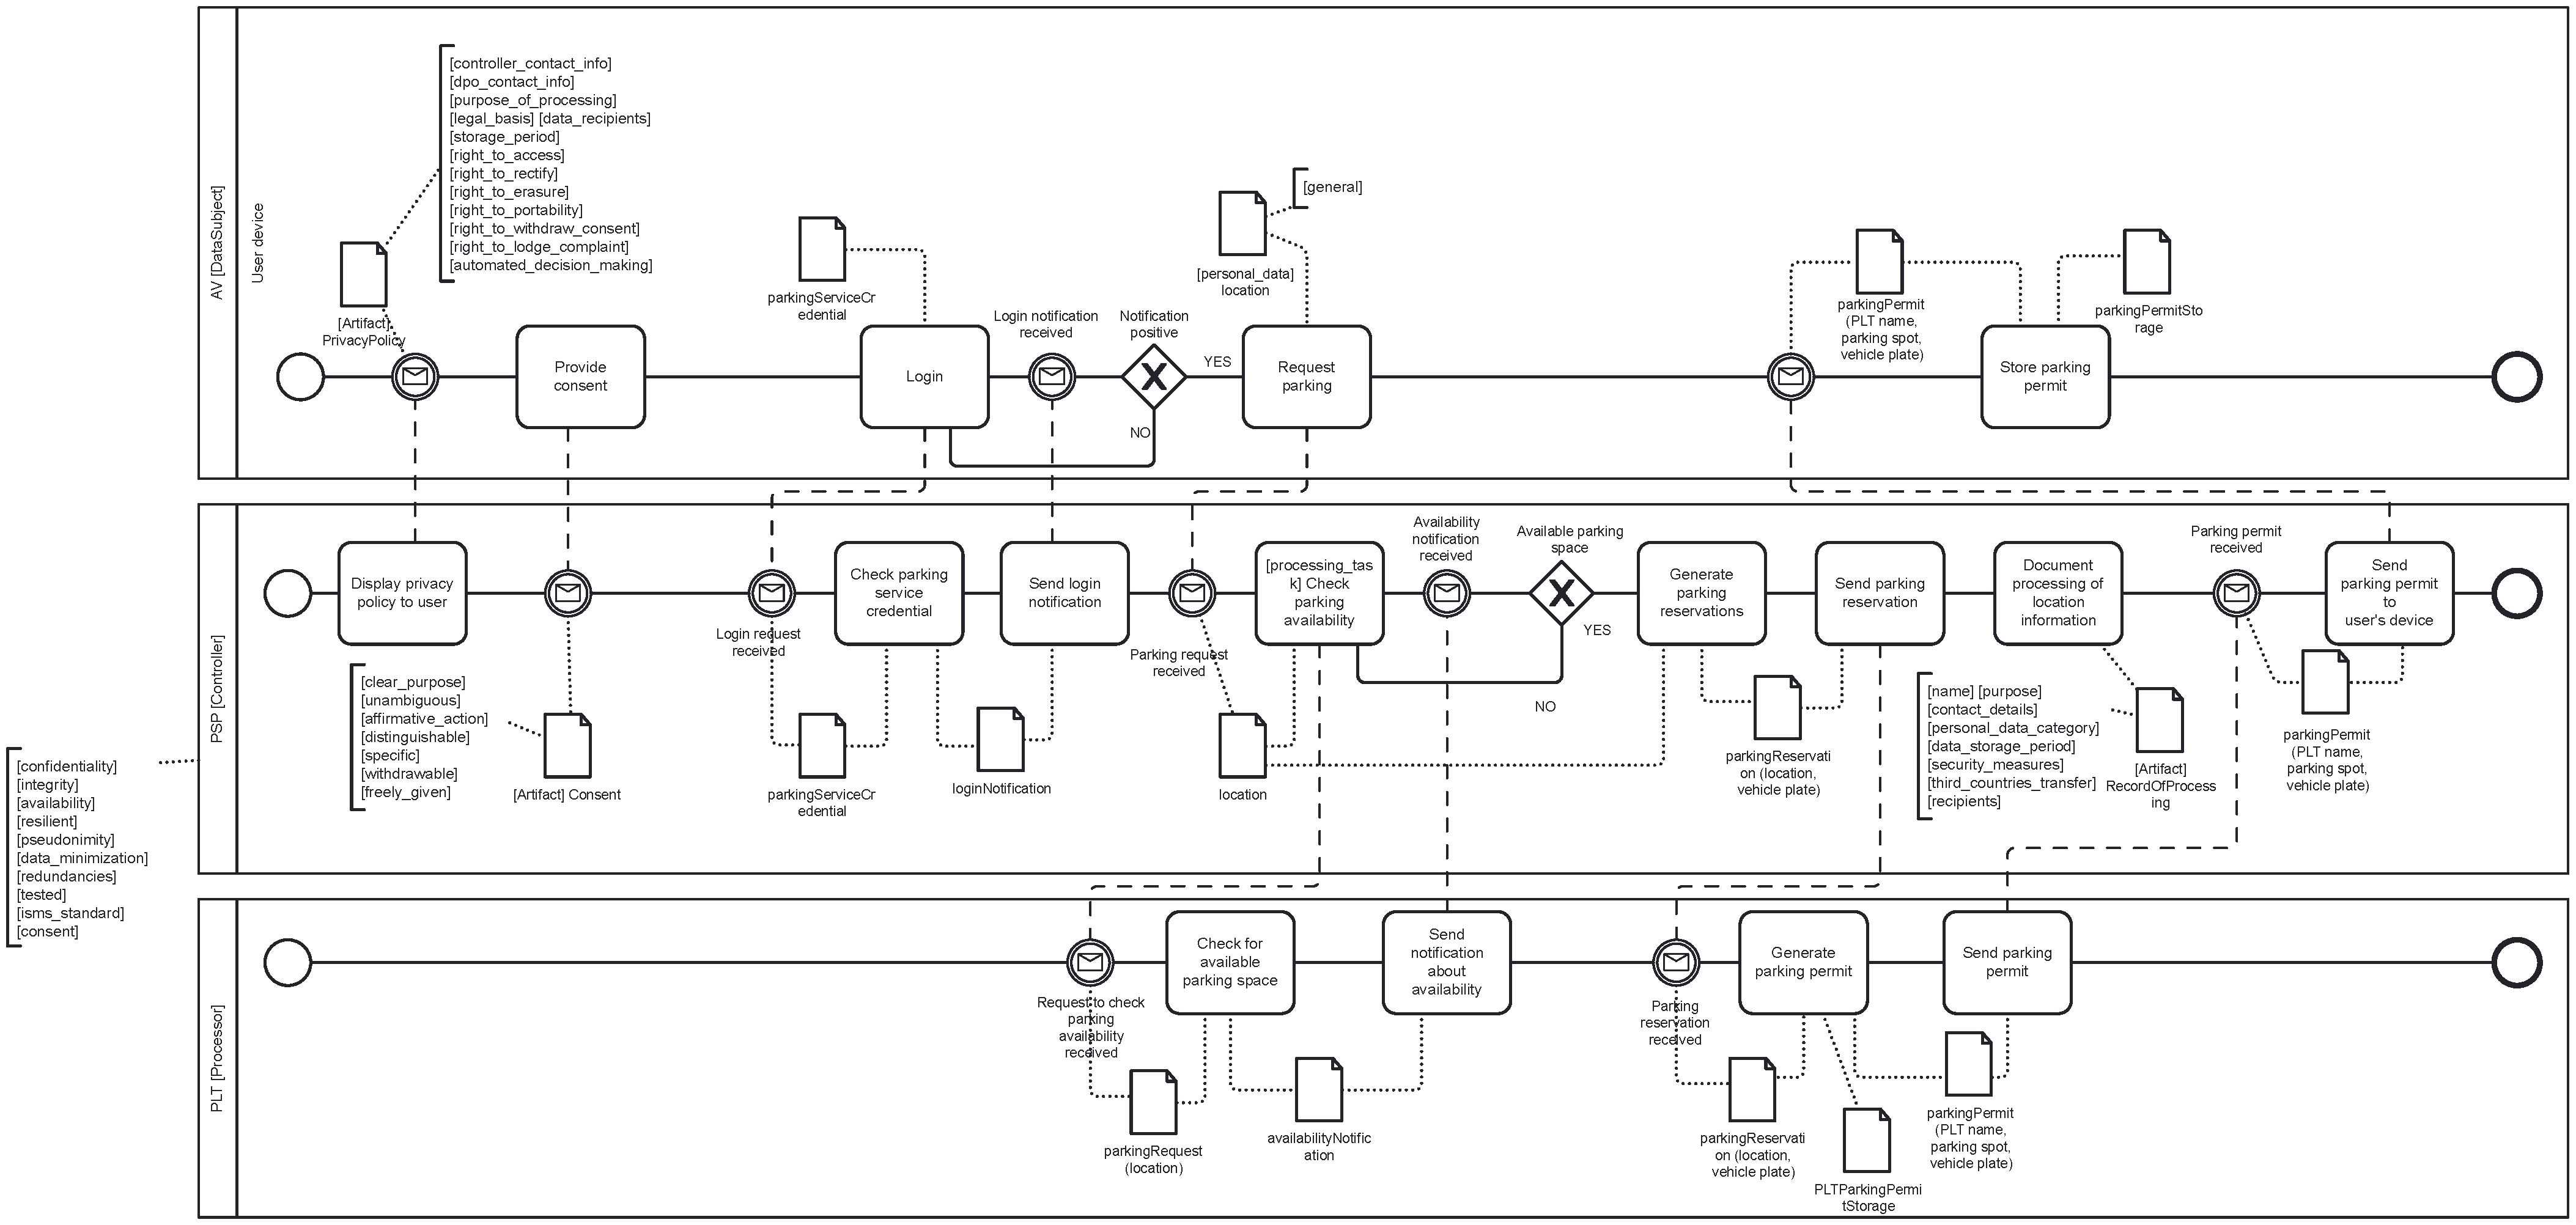
\includegraphics[height=\textwidth - 137pt]{improved.pdf}
  \caption{Improved BPMN model (with GDPR annotations)}
  \label{fig:improved-model}
\end{center}
\end{figure}

\end{landscape}

After performing a GDPR compliance analysis with the DPO tool on the revised
model, we obtained satisfactory results---all initial shortcomings were
addressed. Figure~\ref{fig:improved-uml} displays the result of the updated
evaluation.

\begin{figure}[!hb]
\begin{center}
  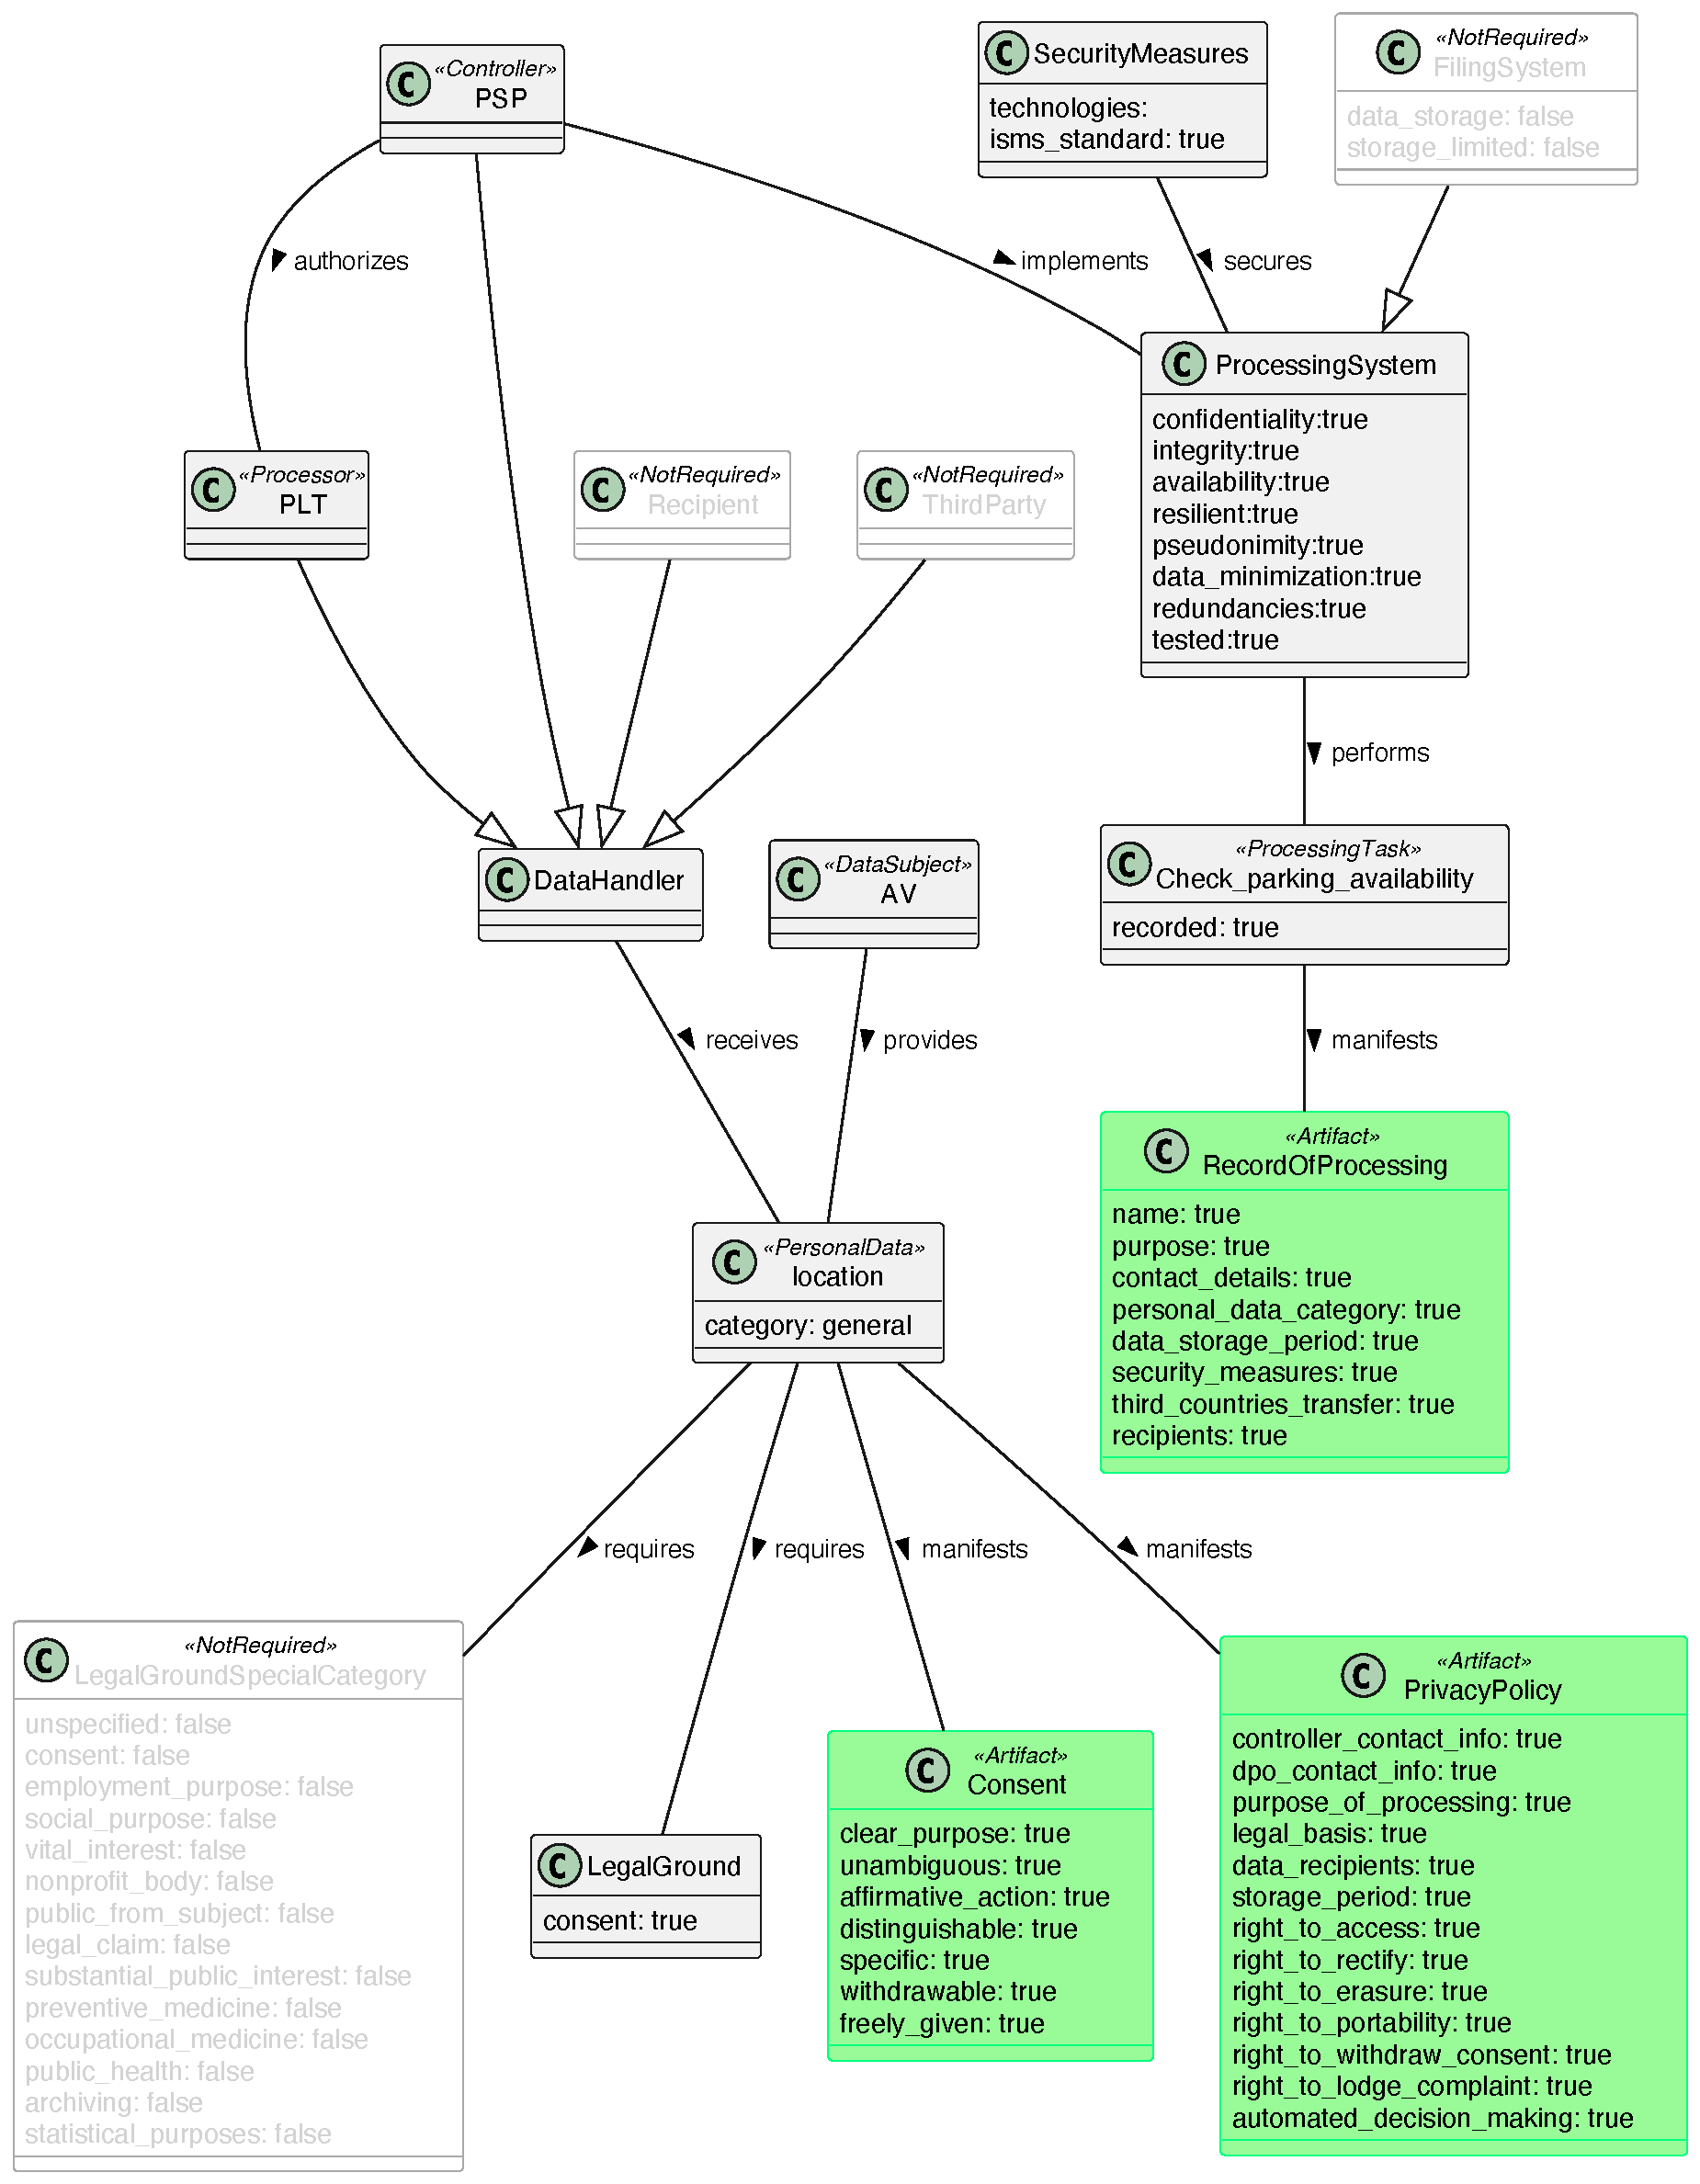
\includegraphics[width=\textwidth - 32pt]{improved-uml.pdf}
  \caption{DPO tool evaluation of the corrected model}
  \label{fig:improved-uml}
\end{center}
\end{figure}

We then re-analysed our improved BPMN model (which is now GDPR compliant with
added annotations) and discovered several shortcomings---namely, the PSP can put
together the customer's identity and the location of their car, even though this
is not needed. For providing the parking service, it is sufficient if only PLT
learns of the parking location, and PSP of the user's identity. Moreover, the
PSP can read the parking permit information even though at this point the PSP
does not need to access these contents.

It becomes clear that data minimisation principles are not followed in the
initial model, and this introduces additional and unnecessary risk of data
leakage. To decrease this risk, we propose the implementation of encryption so
that the PSP can carry some of the user's sensitive data and provided it to the
PLT, but without being able to read and understand the data itself. We further
discuss our recommendations in the next section.
